\documentclass[a4paper, 12pt, twoside]{article}
\usepackage[utf8]{inputenc}		% LaTeX, comprend les accents !
\usepackage[T1]{fontenc}		
\usepackage[francais]{babel}
\usepackage{lmodern}
\usepackage{ae,aecompl}
\usepackage[top=2.5cm, bottom=2cm, 
			left=3cm, right=2.5cm,
			headheight=15pt]{geometry}
\usepackage{graphicx}
\usepackage{eso-pic}	% Nécessaire pour mettre des images en arrière plan
\usepackage{array} 
\usepackage{hyperref}
\usepackage{listings}
\usepackage{verbatim}
%%%%%%%%%%%%%%%%%%%%%%%%%%%%%%%%%%%%%%%%
%    Page de garde (Pagedegarde.tex)   %
%%%%%%%%%%%%%%%%%%%%%%%%%%%%%%%%%%%%%%%%
% Dorian Depriester, 2014

\makeatletter
\def\@ecole{école}
\newcommand{\ecole}[1]{
  \def\@ecole{#1}
}

\def\@entreprise{Nom de l'entreprise}
\newcommand{\entreprise}[1]{
  \def\@entreprise{#1}
}

\def\@datedebut{\today}
\newcommand{\datedebut}[1]{
  \def\@datedebut{#1}
}


\def\@datefin{\today}
\newcommand{\datefin}[1]{
  \def\@datefin{#1}
}



\def\@specialite{Spécialité}
\newcommand{\specialite}[1]{
  \def\@specialite{#1}
}

\def\@ED{\'{E}cole Doctorale}
\newcommand{\ED}[1]{
  \def\@ED{#1}
}

\def\@doctorat{Doctorat}
\newcommand{\doctorat}[1]{
  \def\@doctorat{#1}
}

\def\@adresse{Adresse}
\newcommand{\adresse}[1]{
  \def\@adresse{#1}
}

\def\@directeur{directeur}
\newcommand{\directeur}[1]{
  \def\@directeur{#1}
}

\def\@encadrant{encadrant}
\newcommand{\encadrant}[1]{
  \def\@encadrant{#1}
}
\def\@membrea{Membre}
\newcommand{\membrea}[1]{
  \def\@membrea{#1\\}
}
\def\@membreb{Membre}
\newcommand{\membreb}[1]{
  \def\@membreb{#1\\}
}
\def\@membrec{Membre}
\newcommand{\membrec}[1]{
  \def\@membrec{#1\\}
}
\def\@membred{Membre}
\newcommand{\membred}[1]{
  \def\@membred{#1\\}
}
\def\@membree{Membre}
\newcommand{\membree}[1]{
  \def\@membree{#1\\}
}





\def\@juryb{}{}{}
\newcommand{\juryb}[3]{
  \def\@juryb{#1,	& #2	& #3\\}
}
\def\@juryc{}{}{}
\newcommand{\juryc}[3]{
  \def\@juryc{#1,	& #2	& #3\\}
}
\def\@juryd{}{}{}
\newcommand{\juryd}[3]{
  \def\@juryd{#1,	& #2	& #3\\}
}
\def\@jurye{}{}{}
\newcommand{\jurye}[3]{
  \def\@jurye{#1,	& #2	& #3\\}
}
\def\@juryf{}{}{}
\newcommand{\juryf}[3]{
  \def\@juryf{#1,	& #2	& #3\\}
}
\def\@juryg{}{}{}
\newcommand{\juryg}[3]{
  \def\@juryg{#1,	& #2	& #3\\}
}
\def\@juryh{}{}{}
\newcommand{\juryh}[3]{
  \def\@juryh{#1,	& #2	& #3\\}
}
\def\@juryi{}{}{}
\newcommand{\juryi}[3]{
  \def\@juryi{#1,	& #2	& #3\\}
}
\makeatother

\newcommand\BackgroundPic{%
	\put(0,0){%
		\parbox[b][\paperheight]{\paperwidth}{%
			\includegraphics[height=0.45\paperheight]{bordure.png}%
			\vfill
		}
	}
}
\newcommand\EtiquetteThese{%
	\put(0,0){%
		\parbox[t][\paperheight]{\paperwidth}{%
			\hfill
			%\colorbox{blue}{		
				\begin{minipage}[b]{2em}
					\includegraphics[width=4.0\textwidth]{logo_miage.png}\\					
					%\centering\Huge\textcolor{white}{M\\I\\A\\G\\E\\}
					\vspace{0.2cm}
				\end{minipage}
			%}
		}
	}
}

\makeatletter
\newcommand{\pagedegarde}{
\newgeometry{top=2.5cm, bottom=1cm, left=2cm, right=1cm}
\AddToShipoutPicture*{\BackgroundPic}
%\AddToShipoutPicture*{\EtiquetteThese}
  \begin{titlepage}
  \centering
      
\includegraphics[width=0.6\textwidth]{logo_Paris_Nanterre_couleur_RVB.png}
      \hfill
      $\ $\\
      %\includegraphics[width=0.20\textwidth]{logo_entreprise.png}\\
    \vspace{1cm}
      {\Large Licence CMI-D3S}\\
    \vspace{1cm}
      {\huge 
      	{\bfseries Rapport}\\
    \vspace{0.5cm}}
      	$\ $\\
    \vspace{1cm}
   		
    \vspace{1cm}
    	{\huge\color[rgb]{0,0,1} \bfseries{\@title}}\\
    \vspace{0.5cm}
    %{\bfseries Entreprise d'accueil : \@entreprise}\\
    {\bfseries \@datedebut}\\
    %	{\Large{\bfseries Spécialité doctorale ``\@specialite''}}\\
    \vspace{2cm}
    $\ $\\
    \vspace{0.5cm}
    $\ $\\
    \vspace{0.5cm}
    %	le \@date \\
    \vfill
     %  {\LARGE \color[rgb]{0,0,1} \bfseries{\@title}} \\
    %\vfill
      %  Directeur de thèse : {\bfseries \@directeur}\\
       % Co-encadrant de thèse : {\bfseries \@encadrant}\\
    %\vfill
	\begin{tabular}{>{\bfseries}lll}
		\large Membres du groupe\\
		\vspace{0.15cm}\\
		\@membrea
		\@membreb
		\@membrec
		\@membred
		\@membree
		%\@jurye
		%\@juryf
		%\@juryg
		%\@juryh
		%\@juryi
	\end{tabular}
	%\includegraphics[width=0.20\textwidth]{logo_entreprise.png}\
	\vfill
	
	%\@adresse
  \end{titlepage}




\restoregeometry  
}



\title{Analyse socio-démographique 92}
\entreprise{Le nom de votre entreprise}
\datedebut{23 décembre 2024}




\membrea{Ristic Charlotte}
\membreb{Lafay Mathilde}
\membrec{}
\membred{}
\membree{}



\begin{document}
\pagedegarde

\tableofcontents
\newpage


\section{Généralités}

\subsection{Environnement de travail}

Dans le cadre de ce projet, nous avons utilisé l'éditeur de code Visual Studio Code (VS Code) avec un environnement Linux via WSL2. Par ailleurs, l'extension Live Share nous a permis de collaborer en simultané sur les fichiers, facilitant ainsi le suivi mutuel des modifications apportées au code et garantissant une cohérence dans les méthodes employées.

\subsection{Structure du projet}

Le projet est structuré comme suit :
\begin{itemize}
    \item \textbf{Un fichier \texttt{Optimal}} : Ce fichier contient la résolution brute-force du problème, qui énumère toutes les solutions possibles à partir des sous-ensembles de l’ensemble principal.
    \item \textbf{Un fichier \texttt{Glouton}} : Un algorithme glouton qui permet de sélectionner une collection d'ensemble solution en choisissant à chaque itération, l'ensemble qui couvre le plus d'éléments parmi ceux non encore couverts.
    \item \textbf{Les bibliothèques \texttt{tools.h} et \texttt{tools.c}} : Ces fichiers intègrent des fonctions supplémentaires, notamment pour faciliter la lecture de la matrice.
    \item \textbf{Un fichier \texttt{Makefile}} : Ce fichier précise les règles de compilation. Pour compiler, il suffit de se placer dans le répertoire du projet, puis d'exécuter la commande \texttt{make}. Ensuite, selon l'algorithme souhaité, on exécute soit \texttt{./optimal}, soit \texttt{./glouton}. Enfin, la commande \texttt{make clean} permet de nettoyer les fichiers générés.
\end{itemize}

\section{Présentation de l'algorithme optimal}

\subsection{Définition}

Cet algorithme vise à déterminer tous les sous-ensembles possibles qui couvrent l’ensemble des 
éléments de l'univers \( U \). Nous utilisons la matrice présentée dans l'énoncé pour représenter 
ces sous-ensembles et leurs relations.

\subsection{Notre démarche}

Dans un premier temps, nous avons envisagé de sommer les lignes de la matrice 
jusqu'à obtenir un sous-ensemble dont tous les éléments soient supérieurs ou égaux à 1. 
Un tel résultat indique que l’ensemble est entièrement couvert, c'est-à-dire que tous les 
éléments de \( U \) sont présents dans les sous-ensembles sélectionnés.

Dans un second temps, nous avons changé d’approche en cherchant à parcourir les sous-ensembles 
en commençant par ceux dont le premier élément est 1, puis en poursuivant jusqu’au premier 0. 
À ce stade, nous comparions les sous-ensembles entre eux, en cherchant un 1 dans les positions 
des 0, et en continuant jusqu’à obtenir une couverture complète. 

Finalement, nous avons opté pour une méthode consistant à créer chaque combinaison d'ensemble possible
et à vérifier si celui-ci était solution, plutôt que de chercher directement la solution.
Chaque ensemble est comparé à un autre. S'il est solution, on l'affiche. Puis dans tous les cas, on Continue
les comparaisons en traitant combinant ces deux ensembles afin de le traiter comme un unique ensemble.
De cette manière, nous réduisons progressivement le nombre d'ensembles et avons un 
nombre limité de comparaisons, en ne manipulant toujours que deux sous-ensembles à la fois. 
Ce processus se répète jusqu'à obtenir une couverture complète.

Cette approche nous permet de traiter l’ensemble des sous-ensembles solutions comme un tout, simplifiant ainsi les comparaisons.

\subsection{Explication de l'algorithme}

L'algorithme optimal consiste à explorer toutes les combinaisons possibles de sous-ensembles pour trouver une couverture minimale de l'univers \( U \). Voici les principales étapes de l'algorithme :

\begin{itemize}
    \item Générer toutes les collections d'ensembles possibles de l'univers \( U \).
    \item Pour chaque sous-ensemble, vérifier si la somme des éléments dans les sous-ensembles 
	donne une couverture complète de l'univers.
	\item A chaque itération, on rappelle notre fonction de génération de combinaison, qui va garder notre collection et lui ajouter
	l'ensemble suivant et le tester à nouveau (et ainsi de suite...)
    \item Continuer jusqu'à ce que toutes les combinaisons aient été explorées.
\end{itemize}

Cet algorithme est coûteux en termes de temps d'exécution car il nécessite d'explorer toutes les combinaisons possibles (complexité exponentielle), mais il garantit de trouver la solution optimale.

\subsection{Exemple d'exécution}


Prenons un exemple où l'univers \( U \) est constitué de 7 éléments :

\[
U = \{1, 2, 3, 4, 5, 6, 7\}
\]

et les sous-ensembles disponibles sont :

\[
S = \{A, B, C, D, E, F\}
\]

avec les définitions suivantes :\\
\begin{align*}
A &= \{1, 4, 7\} \\
B &= \{1, 4\} \\
C &= \{4, 5, 7\} \\
D &= \{3, 5, 6\} \\
E &= \{2, 3, 6, 7\} \\
F &= \{2, 7\}
\end{align*}

L'algorithme optimal va explorer toutes les combinaisons possibles de sous-ensembles pour trouver 
une couverture complète de \( U \).

\begin{figure}[h]  % Le flottant pour gérer les images
    \centering  % Centrer l'image
    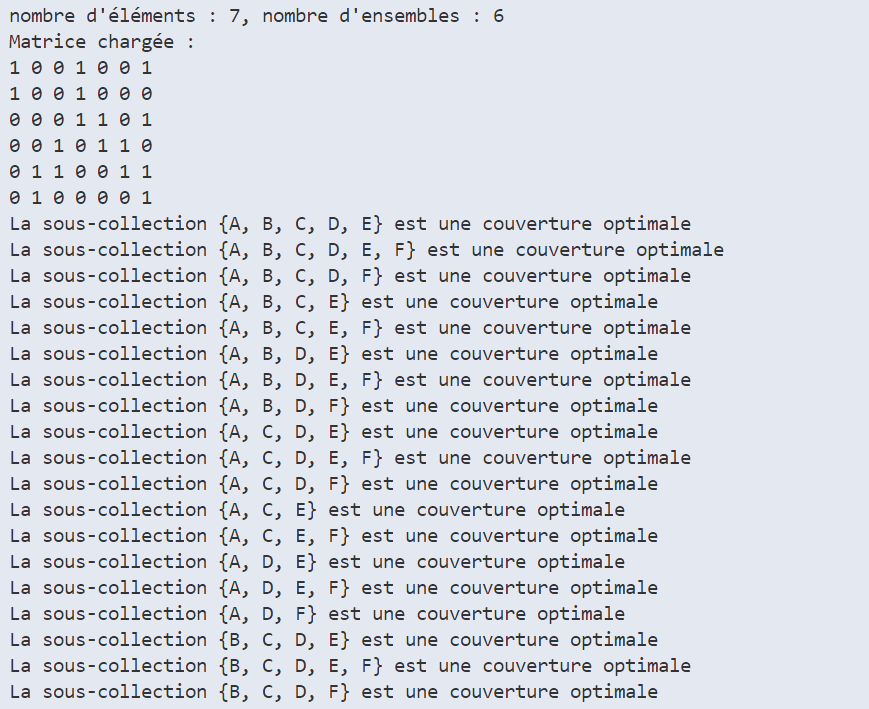
\includegraphics[width=0.5\textwidth]{./optimal.png}  % Lier l'image et définir la taille
    \caption{Exécution brute force}
    \label{fig:exemple_image}  % Label pour faire référence à l'image
\end{figure}

\section{Présentation de l'algorithme glouton}

\subsection{Définition}

L'algorithme glouton vise à simplifier le problème en sélectionnant, à chaque étape, une solution optimale locale, 
ici le sous-ensemble qui maximise le nombre d’éléments non encore couverts.

\subsection{Notre démarche}

Nous avons mis en place une boucle qui identifie, à chaque itération, le sous-ensemble maximisant 
le nombre d'éléments non couverts. Pour ce faire, nous avons utilisé une fonction permettant de compter 
les éléments non encore couverts. On sélectionne celui avec le maximum d'éléments. Une fois un sous-ensemble sélectionné,
il est ajouté à la solution et ses éléments sont considérés comme couverts.

Ce processus est répété jusqu'à ce que tous les éléments de l'univers \( U \) soient couverts.

\subsection{Explication de l'algorithme}

L'algorithme glouton fonctionne en suivant les étapes suivantes :

\begin{itemize}
    \item Initialiser un ensemble de couverture vide.
    \item Tant que tous les éléments de \( U \) ne sont pas couverts :
    \begin{itemize}
        \item Identifier le sous-ensemble avec le plus grand nombre d'éléments non encore couverts.
        \item Ajouter ce sous-ensemble à la couverture.
        \item Marquer les éléments de ce sous-ensemble comme couverts.
    \end{itemize}
    \item Répéter jusqu'à ce que tous les éléments soient couverts.
\end{itemize}

Bien que cet algorithme ne garantisse pas de trouver la solution optimale, il est souvent plus rapide que l'algorithme optimal.

\subsection{Exemple d'exécution}

Prenons le même univers et les mêmes ensembles que dans la partie 2.4 :

\begin{figure}[h]  % Le flottant pour gérer les images
    \centering  % Centrer l'image
    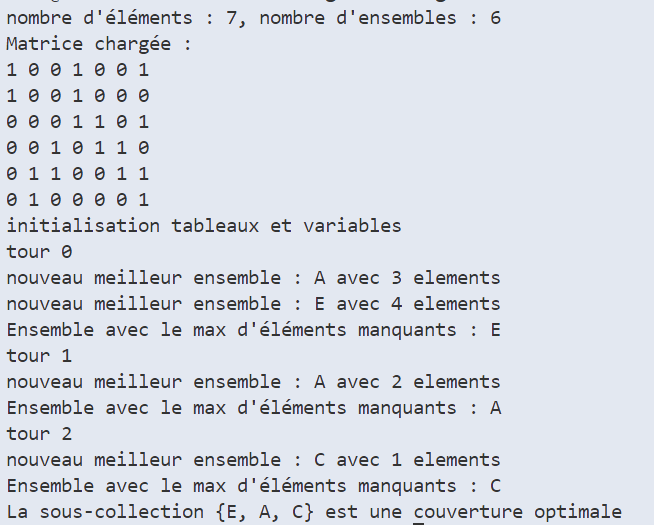
\includegraphics[width=0.5\textwidth]{./glouton.png}  % Lier l'image et définir la taille
    \caption{Exécution algorithme glouton}
    \label{fig:exemple_image}  % Label pour faire référence à l'image
\end{figure}

\end{document}
